\documentclass{article}
\usepackage{tikz}
\usetikzlibrary{arrows.meta, patterns}
\usepackage[margin=0.6in]{geometry}

\begin{document}

% tau_HIGH running ALONE (no interference), one job, release t=0,
% deadline t=30000us (period=deadline=30000). x-axis unit: 1 TikZ unit =
% 1000us, true to scale up to 9.5 (9500us, where all activity ends); the
% axis is broken (zigzag) after that since nothing happens between
% completion and the deadline at 30000us -- the gap is compressed, not to
% scale, purely so the deadline can still be marked on the same figure.
% Derived by hand-simulating DAG-dependency-respecting execution from the
% real core assignment each allocator actually produced (verified against
% the compiled src/dru.cpp / src/tdta.cpp).

\newcommand{\ganttaxis}[1]{
    \draw[thick] (0,#1) -- (9.5,#1);
    \draw[thick] (9.5,#1-0.08) -- (9.7,#1+0.08);
    \draw[thick] (9.6,#1-0.08) -- (9.8,#1+0.08);
    \draw[-{Stealth[length=2mm]}, thick] (9.8,#1) -- (11.3,#1);
}

% ---------------- Figure (a): WF+DRU ----------------
\begin{figure}[tb]
\centering
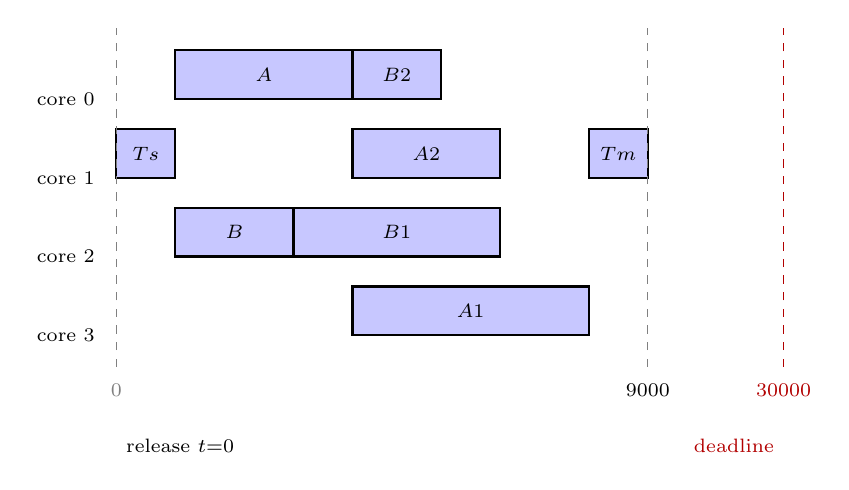
\begin{tikzpicture}[
    x=0.75cm, y=1cm,
    block/.style={fill=blue!22, draw=black, thick},
    tick/.style={font=\scriptsize},
    lbl/.style={font=\scriptsize}
]
    \def\rowh{0.62}
    \foreach \y/\name in {3/core 0, 2/core 1, 1/core 2, 0/core 3} {
        \ganttaxis{\y}
        \node[lbl, anchor=east] at (-0.2,\y) {\name};
    }

    % core0: A[1000,4000], B2[4000,5500]
    \draw[block] (1,3) rectangle ++(3,\rowh)   node[midway,lbl] {$A$};
    \draw[block] (4,3) rectangle ++(1.5,\rowh) node[midway,lbl] {$B2$};
    % core1: Ts[0,1000], A2[4000,6500], Tm[8000,9000]
    \draw[block] (0,2) rectangle ++(1,\rowh)   node[midway,lbl] {$Ts$};
    \draw[block] (4,2) rectangle ++(2.5,\rowh) node[midway,lbl] {$A2$};
    \draw[block] (8,2) rectangle ++(1,\rowh)   node[midway,lbl] {$Tm$};
    % core2: B[1000,3000], B1[3000,6500]
    \draw[block] (1,1) rectangle ++(2,\rowh)   node[midway,lbl] {$B$};
    \draw[block] (3,1) rectangle ++(3.5,\rowh) node[midway,lbl] {$B1$};
    % core3: A1[4000,8000]
    \draw[block] (4,0) rectangle ++(4,\rowh)   node[midway,lbl] {$A1$};

    \draw[dashed, gray] (0,-0.4) -- (0,3.9);
    \node[tick, gray] at (0,-0.7) {$0$};
    \draw[dashed, gray] (9,-0.4) -- (9,3.9);
    \node[tick] at (9,-0.7) {$9000$};
    \draw[dashed, red!70!black] (11.3,-0.4) -- (11.3,3.9);
    \node[tick, red!70!black] at (11.3,-0.7) {$30000$};

    \node[lbl, anchor=west] at (0,-1.4) {release $t{=}0$};
    \node[lbl, red!70!black, anchor=east] at (11.3,-1.4) {deadline};
\end{tikzpicture}
\caption{$\tau_{\mathrm{HIGH}}$ running alone under \textbf{WF+DRU}:
release at $t{=}0$, completes at $t{=}9000\,\mu s$, deadline at
$t{=}30000\,\mu s$ (axis broken after $9500\,\mu s$ -- nothing happens
between completion and the deadline). Every subtask placed on its own
core except $\{A,B2\}$ on core~0, $\{Ts,A2,Tm\}$ on core~1, and
$\{B,B1\}$ on core~2.}
\label{fig:gantt-wfdru-single}
\end{figure}

% ---------------- Figure (b): TDTA ----------------
\begin{figure}[tb]
\centering
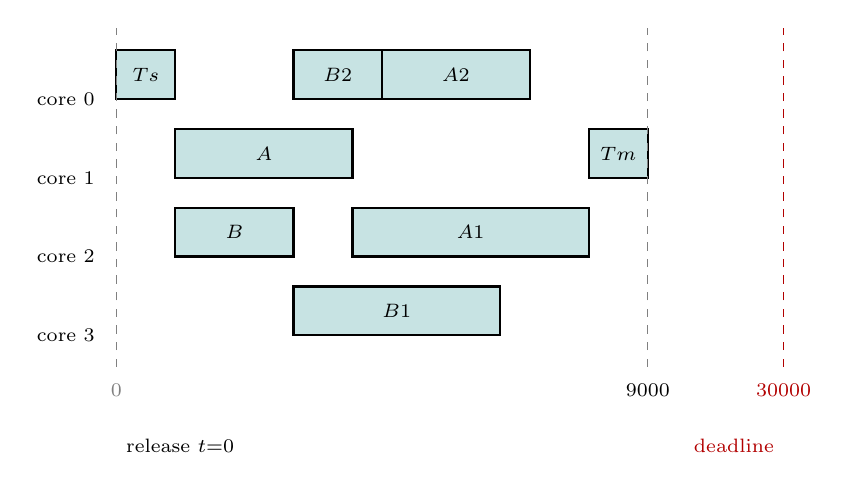
\begin{tikzpicture}[
    x=0.75cm, y=1cm,
    block/.style={fill=teal!22, draw=black, thick},
    tick/.style={font=\scriptsize},
    lbl/.style={font=\scriptsize}
]
    \def\rowh{0.62}
    \foreach \y/\name in {3/core 0, 2/core 1, 1/core 2, 0/core 3} {
        \ganttaxis{\y}
        \node[lbl, anchor=east] at (-0.2,\y) {\name};
    }

    % core0: Ts[0,1000], B2[3000,4500], A2[4500,7000]
    \draw[block] (0,3) rectangle ++(1,\rowh)   node[midway,lbl] {$Ts$};
    \draw[block] (3,3) rectangle ++(1.5,\rowh) node[midway,lbl] {$B2$};
    \draw[block] (4.5,3) rectangle ++(2.5,\rowh) node[midway,lbl] {$A2$};
    % core1: A[1000,4000], Tm[8000,9000]
    \draw[block] (1,2) rectangle ++(3,\rowh)   node[midway,lbl] {$A$};
    \draw[block] (8,2) rectangle ++(1,\rowh)   node[midway,lbl] {$Tm$};
    % core2: B[1000,3000], A1[4000,8000]
    \draw[block] (1,1) rectangle ++(2,\rowh)   node[midway,lbl] {$B$};
    \draw[block] (4,1) rectangle ++(4,\rowh)   node[midway,lbl] {$A1$};
    % core3: B1[3000,6500]
    \draw[block] (3,0) rectangle ++(3.5,\rowh) node[midway,lbl] {$B1$};

    \draw[dashed, gray] (0,-0.4) -- (0,3.9);
    \node[tick, gray] at (0,-0.7) {$0$};
    \draw[dashed, gray] (9,-0.4) -- (9,3.9);
    \node[tick] at (9,-0.7) {$9000$};
    \draw[dashed, red!70!black] (11.3,-0.4) -- (11.3,3.9);
    \node[tick, red!70!black] at (11.3,-0.7) {$30000$};

    \node[lbl, anchor=west] at (0,-1.4) {release $t{=}0$};
    \node[lbl, red!70!black, anchor=east] at (11.3,-1.4) {deadline};
\end{tikzpicture}
\caption{The same $\tau_{\mathrm{HIGH}}$ running alone under \textbf{TDTA}:
release at $t{=}0$, completes at $t{=}9000\,\mu s$ -- identical
completion time to WF+DRU here, since $A1$ (the single largest subtask,
$4000\,\mu s$) sits on its own exclusive core under both strategies and
dominates the critical path either way. What differs is the core
\emph{mapping}: $\{Ts,A2,B2\}$ share core~0, $\{B,A1\}$ share core~2 (not
$\{A,B2\}$/$\{B,B1\}$ as under WF+DRU). With only one task in the system
there is no interference to benefit from yet -- that only shows up once a
second, lower-priority task shares these same cores (see the
HIGH/LOW interference figures).}
\label{fig:gantt-tdta-single}
\end{figure}

\end{document}
